\documentclass{article}
\usepackage[utf8]{inputenc}
\usepackage{hyperref}
\usepackage[margin=1.0in]{geometry}
\usepackage{xcolor}
\usepackage{pgfplots}
\usepgfplotslibrary{external}
\usepackage{gensymb}
\usepackage{amsmath}
\usepackage{tikz}
\usetikzlibrary{shapes, arrows.meta, positioning}
\tikzexternalize
\DeclareMathOperator{\proj}{proj}
\newcommand{\vct}{\mathbf}
\newcommand{\vctproj}[2][]{\proj_{\vct{#1}}\vct{#2}}

\title{Spinning Donut}
\author{DANIEL YANG}
\date{March 2022}

\begin{document}

\maketitle

\section{Introduction}
\begin{flushleft}
This project was based on a \href{https://www.youtube.com/watch?v=DEqXNfs_HhY} {\textcolor{blue}{video}} by Lex Fridman about a donut shaped C code written by Andy Sloane, link to the original article \href{https://www.a1k0n.net/2011/07/20/donut-math.html}{\textcolor{blue}{here}}. This project was my attempt to recreate the results based only on the video without looking at any of the original code by Andy Sloane. In this document, I will explain all of the math that I used and the structure of my own implementation of the spinning donut. The character set used to render the donut was exactly the same as the original so that I could easily compare how close my program got to the original. Here is a link to the Github repo with my code: \url{https://github.com/loltyler1dotcom-discount-code-alpha/Projects}. The code is in the folder titled "Spinning Donut."
\end{flushleft}

\section{Torus Parameterization}
\begin{flushleft}
To parameterize our torus, first imagine a circle of radius 1 centered at the origin in the yz plane.
\end{flushleft}
\centering
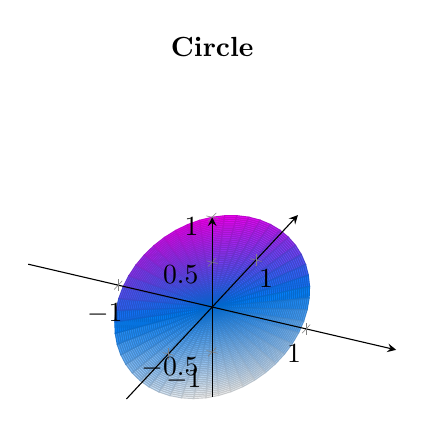
\begin{tikzpicture}
\begin{axis}[
    title=\textbf{Circle},
    axis equal, axis on top,
    axis lines = center,
    colormap/cool,
]
\addplot3 [
        surf,
        domain=0:360, %sets range for x
        y domain=0:1,
        samples=50, %number of samples taken
        ]
(
    {y*sin(x)*cos(45)},
    {y*sin(x)*sin(45)},
    {y*cos(x)}
);

\end{axis}
\end{tikzpicture}

\begin{flushleft}
The circle is tilted at an arbitrary angle from the x axis on the xy plane, $\theta$, and the azimuthal angle is defined by an angle $\phi$. The parameterization of this circle with radius 1 must be: $$C(\phi)=\langle \sin(\phi)\cos(\theta),\sin(\phi)\sin(\theta),\cos(\phi) \rangle$$

where $\theta$ is some constant value. \\
\end{flushleft}

\begin{flushleft}
In order to get a torus, we must have this circle $C(\phi)$ and translate it a constant $R$ distance in the direction of $\theta$ for all $0 \leq \theta \leq 2\pi$. \\
For this program, we will set $R = 2$. To translate the tilted circle in the direction of $\theta$, we simply have to add the x and y components of the vector $\mathbf{R}$. Using basic trigonometry, we get $\mathbf{R} = 2\langle \cos(\theta), \sin(\theta), 0 \rangle$. Adding $\mathbf{R}$ to $C(\phi, \theta)$ where $\theta$ is defined on all $0 \leq \theta \leq 2\pi$, we get our parameterization for the torus: $$G(\phi,\theta) = \langle (2+\sin(\phi))\cos(\theta),(2+\sin(\phi))\sin(\theta),\cos(\phi) \rangle$$
This ends up giving us a surface that looks like this:
\end{flushleft}
\centering
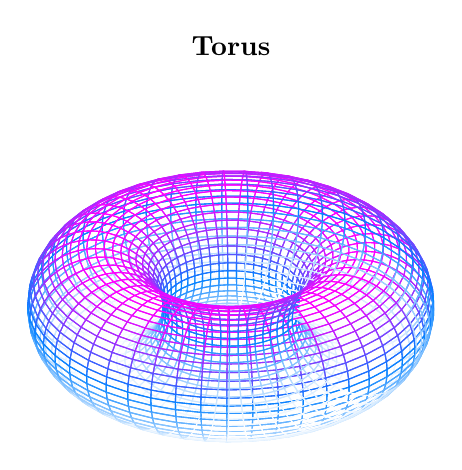
\begin{tikzpicture}
\begin{axis}[
    title=\textbf{Torus},
    hide axis, axis equal,
    colormap/cool,
]
\addplot3 [
        mesh,
        domain=0:360, %sets range for x
        y domain=0:360,
        samples=50, %number of samples taken
        ]
(
    {(2+sin(x))*cos(y)},
    {(2+sin(x))*sin(y)},
    {cos(x)}
);

\end{axis}
\end{tikzpicture}

\section{Transformations}
\begin{flushleft}
To rotate a point around the x axis, we can first represent that point as a vector $\left(
\begin{array}{c}
    x_1  \\
    y_1  \\
    z_1 \\
\end{array} \right)$ whose tail is attached to and is perpendicular to the x axis. Using the y axis as 0 degrees, $\alpha$ as the angle we need to rotate the point by, and $\theta$ as the original angle the vector makes with the y axis, we can write the coordinates of this vector as:
    $$x_1 = x_1$$ $$y_1 = r\cos(\theta)$$ $$z_1 = r\sin(\theta)$$
We then have the new rotated coordinates:
$$x_2 = x_1$$ $$y_2 = r\cos(\alpha + \theta) = r(\cos(\theta)\cos(\alpha)-\sin(\theta)\sin(\alpha))$$
$$z_2 = r\sin(\alpha + \theta) = r(\sin(\theta)\cos(\alpha)+\cos(\theta)\sin(\alpha))$$

Substituting the previous values for original coordinates, we get $$x_2 = x_1$$ $$y_2 =  y_1\cos(\alpha)-z_1\sin(\alpha)$$
$$z_2 = y_1\sin(\alpha) + z_1\cos(\alpha)$$

We can write this relationship as a transformation matrix $$\mathbf{X} = \left(
\begin{array}{ccc}
    1 & 0 & 0 \\
    0 & \cos(\alpha) & -\sin(\alpha)  \\
    0 & \sin(\alpha) & \cos(\alpha) \\
\end{array} \right)$$ where $\mathbf{X}$ can be multiplied by a vector of 3 dimensions to get a new point rotated about the x axis by some angle $\alpha$. We can repeat this process of using trig identities to solve a system of equations for rotating about the y and z axes by some angle $\beta$ and $\gamma$ to get two transformation matrices $\mathbf{Y}$ and $\mathbf{Z}$. We can then combine these transformation matrices into one transformation matrix:
$$\mathbf{T} = \mathbf{Z} \mathbf{Y} \mathbf{X}$$
$$\mathbf{T} = \left(
\begin{array}{ccc}
    \cos(\beta)\cos(\gamma) & \sin(\alpha)\sin(\beta)\cos(\gamma)-\cos(\alpha)\sin(\gamma) & \cos(\alpha)\sin(\beta)\cos(\gamma)+\sin(\alpha)\sin(\gamma) \\
    \cos(\beta)\sin(\gamma) & \sin(\alpha)\sin(\beta)\sin(\gamma)+\cos(\alpha)\cos(\gamma) & \cos(\alpha)\sin(\beta)\sin(\gamma)-\sin(\alpha)\cos(\gamma) \\
    -\sin(\beta) & \sin(\beta)\cos(\beta) & \cos(\alpha)\cos(\beta) \\
\end{array} \right) $$
\end{flushleft}

\section{Illumination}
\begin{flushleft}
To calculate the illumination of each point on the torus, we can set out viewport to being the xy plane with our normal vector in the positive z direction. We can then project the torus onto the xy plane and then calculate the amount of light that hits our viewport by calculating the projection of the torus' surface normal vector $\vec{N}$ onto the negative unit vector of the viewport $-\vec{n} = \langle 0,0,-1 \rangle$.
\end{flushleft}

\begin{flushleft}
Our parameterization of the torus was $$G(\phi,\theta) = \langle (2+\sin(\phi))\cos(\theta),(2+\sin(\phi))\sin(\theta),\cos(\phi) \rangle$$
In order to get the surface normal vector of this parameterization, we need to take the cross product of the partial derivatives in the positive $\phi$ and $\theta$ directions.
$$\frac{\partial G}{\partial \phi} = \langle \cos(\phi)\cos(\theta), \cos(\phi)\sin(\theta),- \sin(\phi)\rangle$$
$$\frac{\partial G}{\partial \theta} = \langle-(2+\sin(\phi))\sin(\theta),(2+\sin(\phi))\cos(\theta),0\rangle$$
$$\vec{N} = \frac{\partial G}{\partial \phi} \times \frac{\partial G}{\partial \theta}$$
$$\vec{N} = \langle \sin(\phi)\cos(\theta),\sin(\phi)\sin(\theta),\cos(\phi) \rangle$$
To get the magnitude of the surface normal vector in the direction of the negative viewport normal, we project the surface normal vector onto the negative viewport normal.
$$\vctproj[-\vec{n}]{\vec{N}} = \frac{\vec{N} \cdot -\vec{n}}{(-\vec{n})\cdot(-\vec{n})}(-\vec{n})$$
Since $-\vec{n}$ has a magnitude of 1, the expression becomes:
$$\langle 0,0,\cos(\phi) \rangle$$
We want to have our illumination based on the amount of light that hits the xy plane. This can be done by setting our illumination to the negative magnitude of the projection, which will increase the more the surface normal of the torus points towards the -z direction.
$$Ill = -\cos(\phi)$$
\end{flushleft}

\section{Implementation}

\begin{flushleft}
So now that we have all the math worked out and the transformation matrices in place, how can we implement these equations into the program? \\
\textbf{INITIAL} \\
\end{flushleft}
\centering
\tikzstyle{terminator} = [rectangle, draw, text centered, rounded corners, minimum height=2em]
\tikzstyle{process} = [rectangle, draw, text centered, minimum height=2em]
\tikzstyle{decision} = [diamond, draw, text centered, minimum height=2em]
\tikzstyle{data}=[trapezium, draw, text centered, trapezium left angle=60, trapezium right angle=120, minimum height=2em]
\tikzstyle{connector} = [draw, -latex']
\usetikzlibrary{shapes, arrows}
\begin{tikzpicture}[node distance = 2.5cm]
\node [terminator, fill=blue!20] (start) {\textbf{Input (x,y)}};
\node [data, fill=blue!20, below of=start] (undo) {Undo Transformation Matrix};
\node [data, fill=blue!20, below of=undo] (get) {Get $\phi$ and $\theta$ parameters};
\node [data, fill=blue!20, below of=get] (solve) {Solve for $Ill$};
\node [decision, fill=blue!20, below of=solve] (decision) {Valid?};
\node [process, fill=red!20, right of=decision] (error) {Not Found};
\node [process, fill=green!20, below of=decision] (success) {Return Illumination};
\node [terminator, fill=blue!20, below of=success] (end) {\textbf{End}};
\node[draw=none] at (1.15, -9.70) (no) {No};
\node[draw=none] at (0.35, -13.75) (yes) {Yes};
\path [connector] (start) -- (undo);
\path [connector] (undo) -- (get);
\path [connector] (get) -- (solve);
\path [connector] (solve) -- (decision);
\path [connector] (decision) -- (error);
\path [connector] (decision) -- (success);
\path [connector] (error) |- (end);
\path [connector] (success) -- (end);
\end{tikzpicture}
\begin{flushleft}
The way I initially programmed the spinning donut was to have an array of $(x,y)$ coordinates which would represent characters to be displayed on the screen and calculate the illumination directly. There was a big problem with this method in that solving the math was very ass and I wasted a lot of time trying to find an analytical solution to this. The main issue was that since the torus was parameterized, transformed, then projected, calculating the illumination required knowing the original $\phi$ and $\theta$ parameters from before the transformation matrix was applied, which is practically impossible given the large complexity of the transformation matrix.
\end{flushleft}

\begin{flushleft}
\textbf{WORKING} \\
\end{flushleft}
\begin{tikzpicture}[node distance = 2.5cm]
\node [terminator, fill=blue!20] (start) {\textbf{Point Array}};
\node [data, fill=blue!20, below of=start] (apply) {Apply Transformation Matrix};
\node [data, fill=blue!20, below of=apply] (solve) {Solve for $Ill$};
\node [decision, fill=blue!20, below of=solve] (decision) {Valid?};
\node [process, fill=red!20, right of=decision] (error) {Not Found};
\node [process, fill=green!20, below of=decision] (success) {Return Illumination};
\node [terminator, fill=blue!20, below of=success] (end) {\textbf{End}};
\node[draw=none] at (1.2, -7.25) (no) {No};
\node[draw=none] at (0.35, -11.25) (yes) {Yes};
\path [connector] (start) -- (apply);
\path [connector] (apply) -- (solve);
\path [connector] (solve) -- (decision);
\path [connector] (decision) -- (error);
\path [connector] (decision) -- (success);
\path [connector] (error) |- (end);
\path [connector] (success) -- (end);
\end{tikzpicture}

\begin{flushleft}
The solution I decided upon was to have an large array of arrays (a vector of vectors if we are being specific to C++ datatypes) which would keep track of points on the parameterized surface. Instead of calculating the surface normal vector using $(x,y)$ coordinates as inputs, we can just represent the normal vectors as points by adding the normal vector to the vector parameterized by $\phi$ and $\theta$, which can be visualized as attaching the normal vector of each point on the surface to the surface itself. Then, by applying the matrix transformation on both the point on the surface and the point generated by attaching the surface normal onto the point on the surface, we can find the illumination without needing to know the original parameters of the torus.
\end{flushleft}

\begin{flushleft}
Now, we can define a struct for each point:
$$struct\ (point) = \{x,y,z\} \cup \{nx,ny,nz\}$$
where x,y,z represent points on the surface and nx,ny,nz represent the calculated point from the normal vector. \\
We then create an array of these points where:
$$Points[point] = [point_1, point_2, \ldots ,point_n]$$
Then for each item in the array, we apply the transformation matrix on both the x,y,z and on the coordinates of the normal. To calculate the illuminance, we can then subtract z from nz. $$Ill = z - nz$$ 
\end{flushleft}

\begin{flushleft}
At first, I applied the transformation matrix with an angle delta on every frame and overwrote the array $Points[point]$ and loaded the illuminance onto another array storing the values to render to the screen. This came with an issue since float values are truncated so every time the transformation matrix would be applied, some of the data would be lost with the floating point truncation, making the magnitude of the points smaller and smaller every frame, leading to a shrinking effect. To solve this, I instead kept the initial array of non-translated points stored and every frame, I would apply the transformation matrix on the total change in angle from the original using a running total of the angle deltas. This ended up resolving the shrinking donut effect.
\end{flushleft}

\end{document}
